
\documentclass[10pt,english]{article}
\usepackage[bottom=0.8in,margin=0.8in]{geometry}
\geometry{a4paper}
\usepackage[english]{babel}
\usepackage{indentfirst}
\selectlanguage{english}
\usepackage{multicol}
%\usepackage{varioref}% smart page, figure, table, and equation referencing
\usepackage[colorlinks]{hyperref}% hyperlinks [must be loaded after dropping]
\hypersetup{colorlinks,breaklinks,
citecolor = blue,
urlcolor=blue,
linkcolor=blue}
\usepackage[noabbrev]{cleveref}

\usepackage{placeins}
%\usepackage{float}
\usepackage[utf8]{inputenc}



\usepackage{graphicx}

\usepackage{amssymb}
\usepackage{authblk}
\graphicspath{{../Plots/}} % allows figures to be placed in a different folder



\title{\vspace{-20pt}Infinite Cylinder CFD Simulation Verification and Validation}
\author{Kevin R. Moore}
\affil{\vspace{-5pt}Brigham Young University}
\renewcommand\Authands{, }
\date{\vspace{-10pt}\today}

\begin{document}

\maketitle
\vspace{-10pt}
%\section{Project Overview}
   \textbf{The purpose of this study is to demonstrate proficiency in the areas of verification and validation of CFD in light of an open ended problem definition; Explore laminar flow over a cylinder.  I performed this in four steps: First, I developed a simulation according to rules of thumb that validated against experimental data within 1.5\% of the coefficient of drag (\textit{Calculation of Drag Coefficient for Arrays of Emergent Circular Cylinders with Pseudofluid Model} by Cheng).  Second, I changed the mesh density to show grid independence.  Third, I used the chosen new mesh and changed the domain boundary size to show boundary independence.  Fourth, I revisited the temporal and transient solver parameters to verify temporal independence with the changes from the base rule of thumb simulation. }

\vspace{0pt}

\section{Model Overview}

With the objective to model laminar flow over a cylinder, I chose a domain that, based on my previous experience, should have been more than capable of accurately resolving the dynamic forces on the cylinder.  I chose a bullet shaped domain to save some computational expense and started with an inlet radius of 10 diameters.  I chose an exit distance from the cylinder of 30 diameters and a resolved wake distance of 20 diameters.  I grossly over-exaggerated the wake distance and did not change it in this study to remove a variable and enable me to focus on improving my proficiency in verification and validation during a reasonable time scale.  This is also the case on the prism layer mesh around the cylinder.  \Cref{f:domain} gives a visual representation of the domain and \cref{tab:params} gives values for the domain.


%\begin{figure}[htbp]
%\centering
%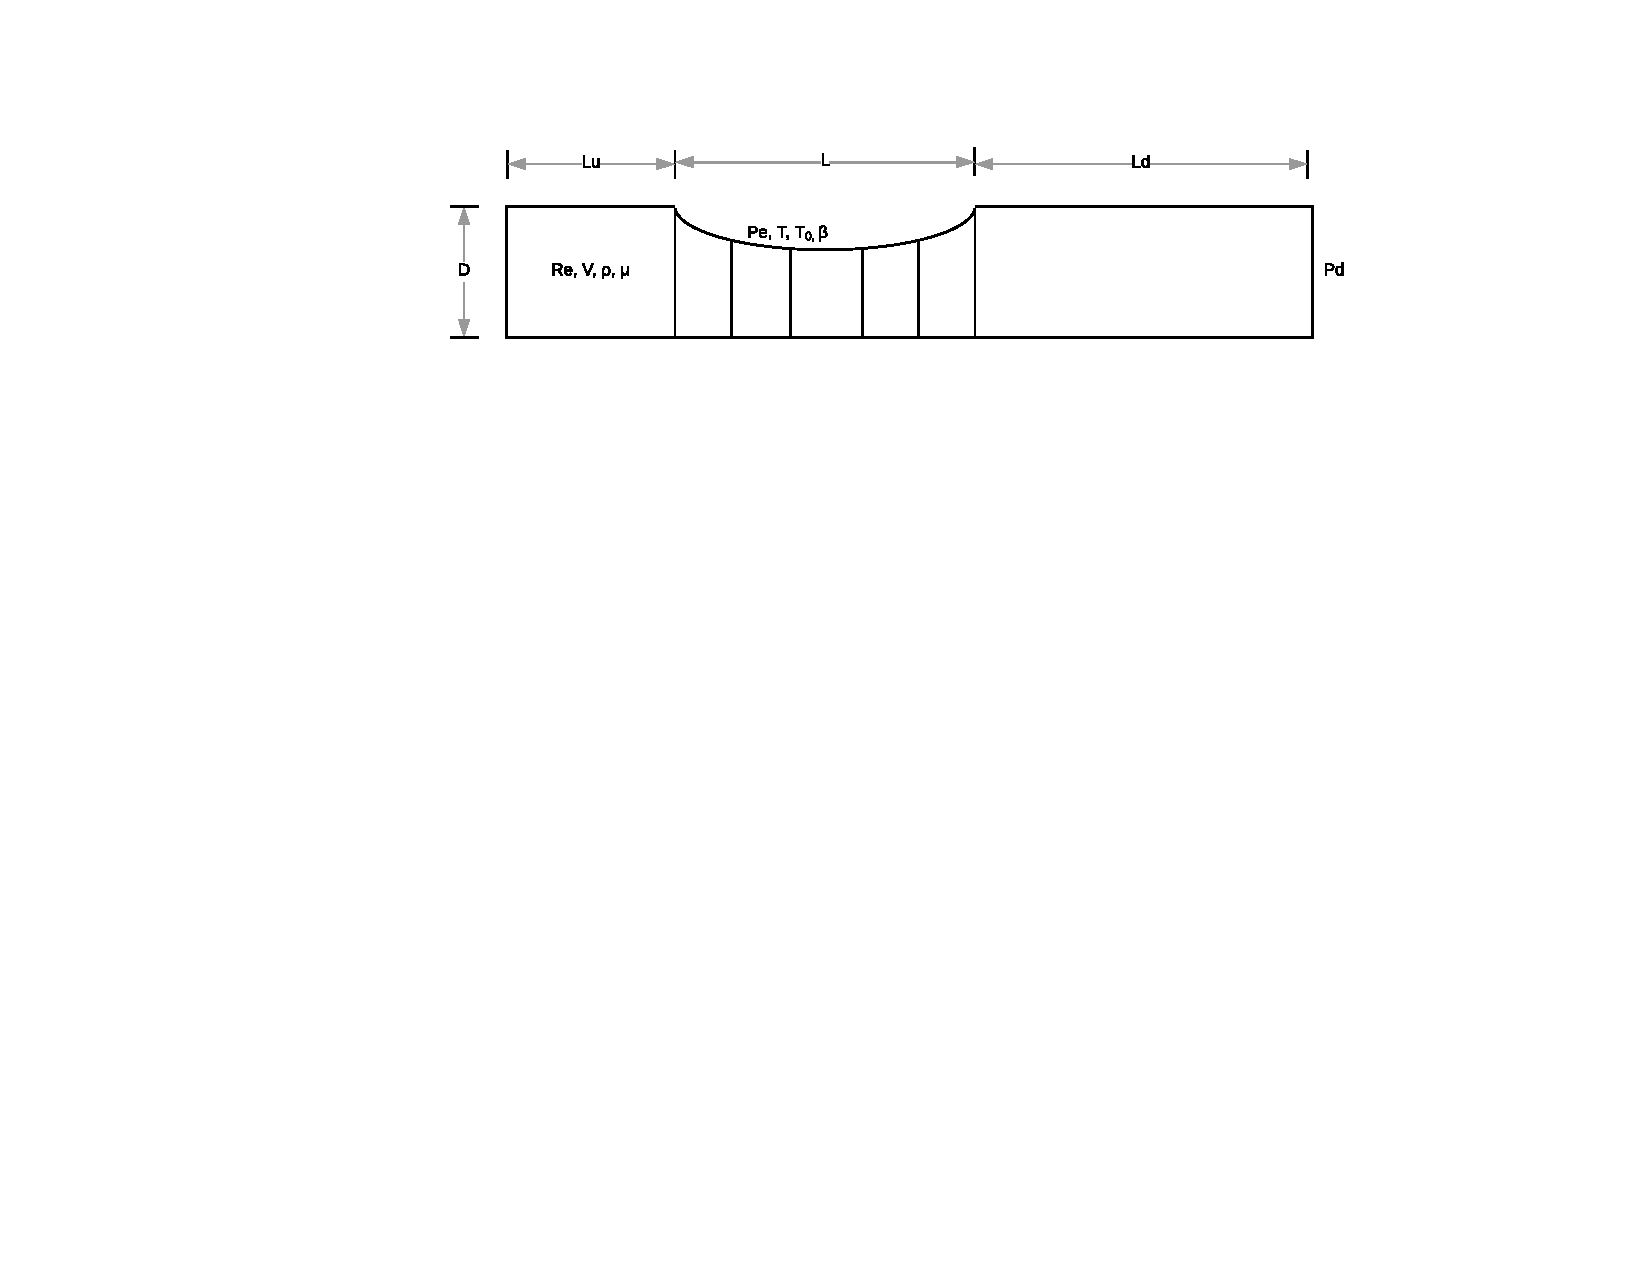
\includegraphics[trim={7.5cm 15.5cm 5.6cm 2.5cm},clip,width=0.95\textwidth]{Adina_Setup}
%\caption{Illustration of the experimental setup and sectioning for meshing, not to scale.}
%\label{f:setup}
%\end{figure}

\begin{figure}[h!]
\centering
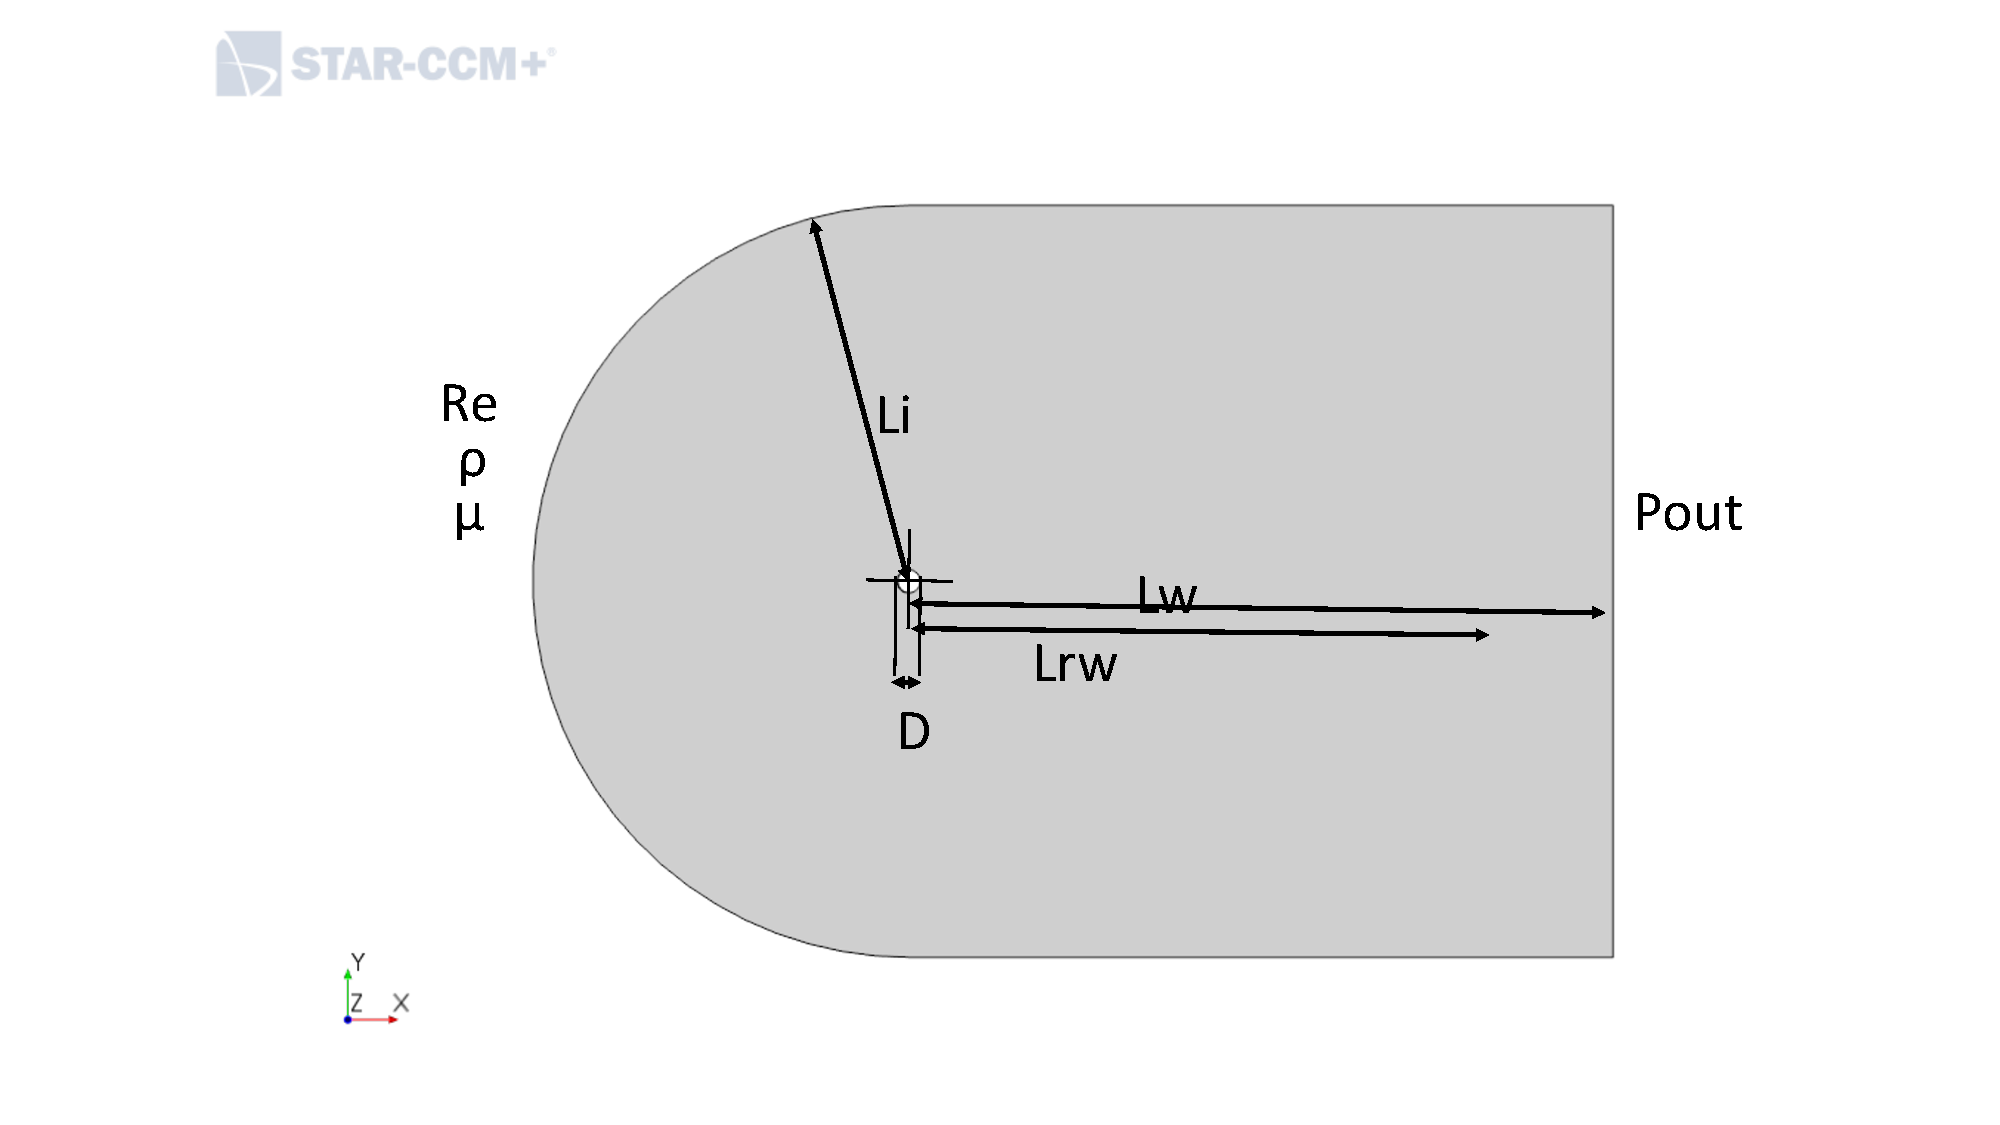
\includegraphics[trim={6.5cm 2.5cm 4.0cm 3cm},clip,width=0.60\textwidth]{domain}
\caption{General domain representation, to scale for the final chosen simulation.}
\label{f:domain}
\end{figure}

\begin{table*}[h]
\vspace{20pt}
\centering
  \begin{tabular}{lcl}
    \textbf{Name} & \textbf{Value} & \textbf{Description}  \\
    D & 0.01 m & Cylinder Diameter  \\
    Li & 10-18 D & Inlet Radius\\
    Lw & 30 D & Outlet Distance\\
    Lrw & 20 D & Resolved Wake Distance\\
    Re & 20, 150 & Reynolds Number (cylinder diameter)\\
    $\rho$  & 1.225 m/kg & Fluid Density\\
    $\mu$  & 1.855 E-5 Pa-s & Fluid Viscosity\\ 
  \end{tabular}
  \caption{Summary of domain geometry and fluid variables.}
  \label{tab:params}
\end{table*}



\vspace{5pt}
\section{Initial Validated Simulation}

Following best practices as described by CD-Adapco, Dr. Ning, and my previous experience, I developed a simulation that validated to within 1.49\% for the Re 150 case and 0.27\% for the Re 20 case.  A plot of the values and the experimental data from Cheng can be seen in \cref{f:val1}.  Due to the nature of the laminar flow, Reynolds number, and mach number, I was able to take advantage of the laminar and incompressible assumptions in the physics conditions.  If I had been modeling flow past Re 1E6, significantly more verification would need to be done to include turbulent effects.


\begin{figure}[htbp]
\centering
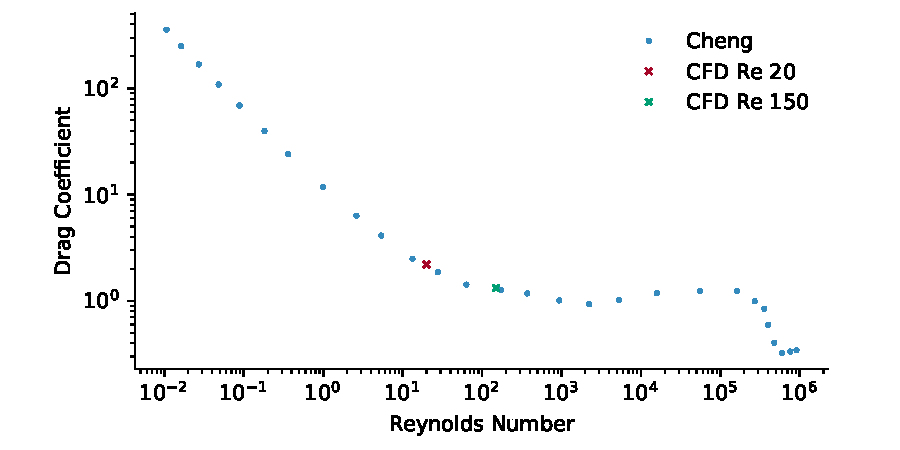
\includegraphics[trim={.0cm .25cm .0cm 0cm},clip,width=0.75\textwidth]{validation}
\vspace{-5pt}
\caption{Initial simulation validation against data from Cheng. Validated to within 1.49\% for the Re 150 case and 0.27\% for the Re 20 case. }
\label{f:val1}
\end{figure}

 I chose an initial inlet radius of 10 diameters, fluid parameters standard for air at sea level, and an inlet velocity to match the required Reynolds number based on the cylinder diameter.  I applied the velocity condition to the front continuous surface of the bullet in the x-direction and used a pressure 0.0 pa exit boundary.  I chose polyhedral elements with prism meshing, a grid base size of 5 diameters, but refined the mesh around the cylinder to have a target size of 0.1 diameters (2\% of the base size).  I chose to refine the wake out to 20 diameters with a 10 degree spread and a relative size of 5\% of the base size.  I found that the default wake refinement was not wide enough in the near-field, so I also added a second wake with a 30 degree spread that extended 3 diameters which gives the meshed domain an arrow like appearance.  Blending of the mesh was done with a 20\% growth rate to the boundaries, which left boundary cells sometimes smaller than the base size.  \Cref{f:mesh05_1} shows the entire meshed domain.
 
 \begin{figure}[h]
\centering
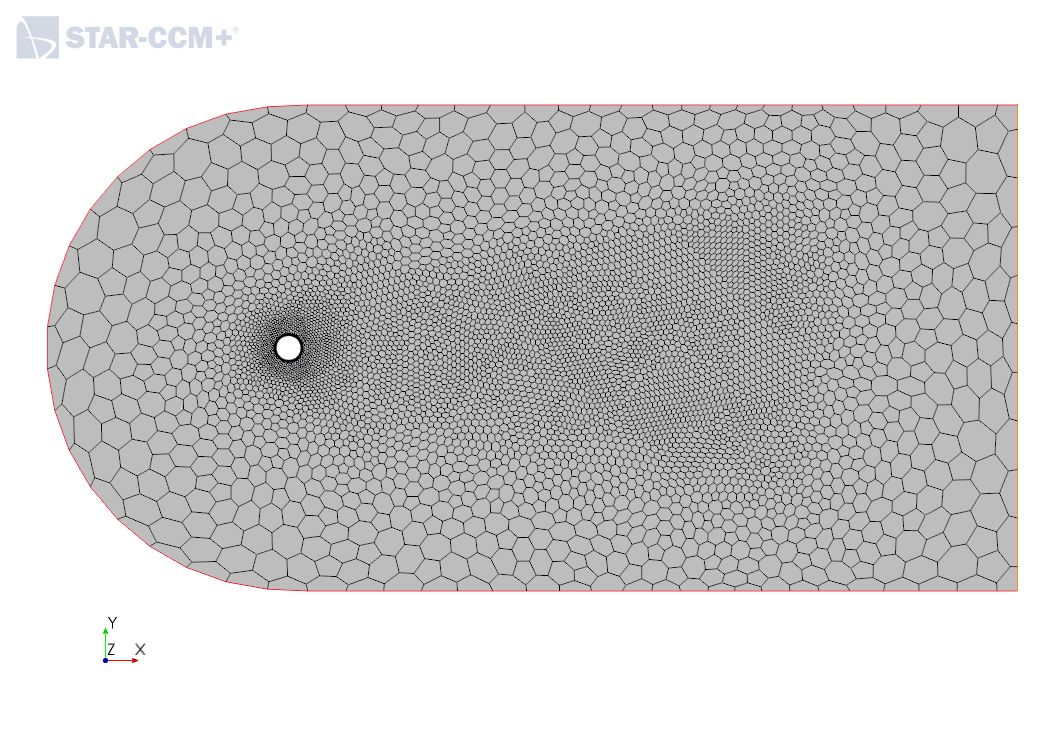
\includegraphics[trim={1.5cm 5cm 1.0cm 3cm},clip,width=0.7\textwidth]{cylinder_2_05_MeshScene2.png}
\vspace{-5pt}
\caption{Initial meshed domain shows widened near wake region to accommodate periodic vortex shedding. }
\label{f:mesh05_1}
\end{figure}

I chose 20 prism layers with a 20\% growth rate, a minimum thickness of 2.5E-4, or enough to satisfy the y+ condition for both Reynolds numbers and amply resolve the boundary layer.  However, while the total thickness of the prism layer was adequate for Re 20, I failed to include enough thickness for Re 150 by a factor of about 2.  This doesn't appear to affect the validation solutions though because of the relatively well refined unstructured mesh and prism layer lateral discretization.  The boundary layer (besides the lateral discretization based on the target surface size) was not investigated based on the intent and time constraints of the project.  The number of cells for this base case, including the prism layers was 6,163 cells. \Crefrange{f:mesh05_2}{f:mesh05_3} show a closer-up image of the cylinder and prism mesh respectively.  


\begin{figure}[h]
\centering
\begin{minipage}{.49\textwidth}
  \centering
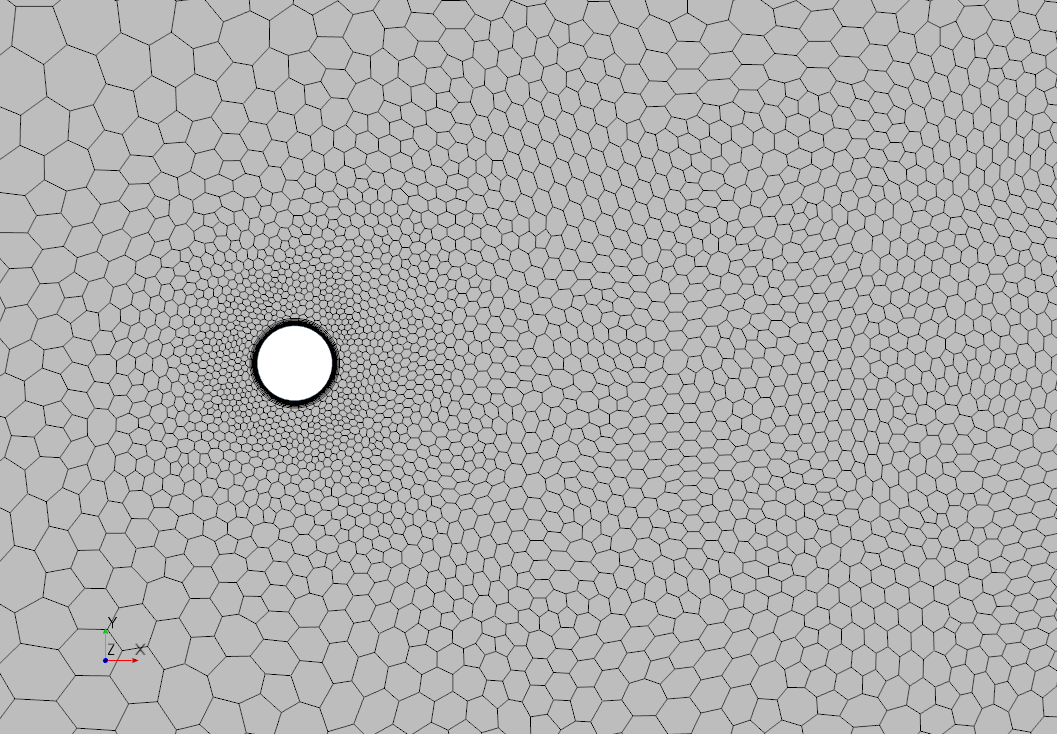
\includegraphics[trim={1.0cm 0cm 1.4cm 0.5cm},clip,width=0.98\textwidth]{cylinder_2_05_MeshScene2_2.png}
%\vspace{-3pt}
\caption{Mesh relatively fine in the regions departing from the cylinder allows for adequate wake refinement.}
\label{f:mesh05_2}
\end{minipage}%
\hspace{5pt}
\begin{minipage}{.49\textwidth}
  \centering
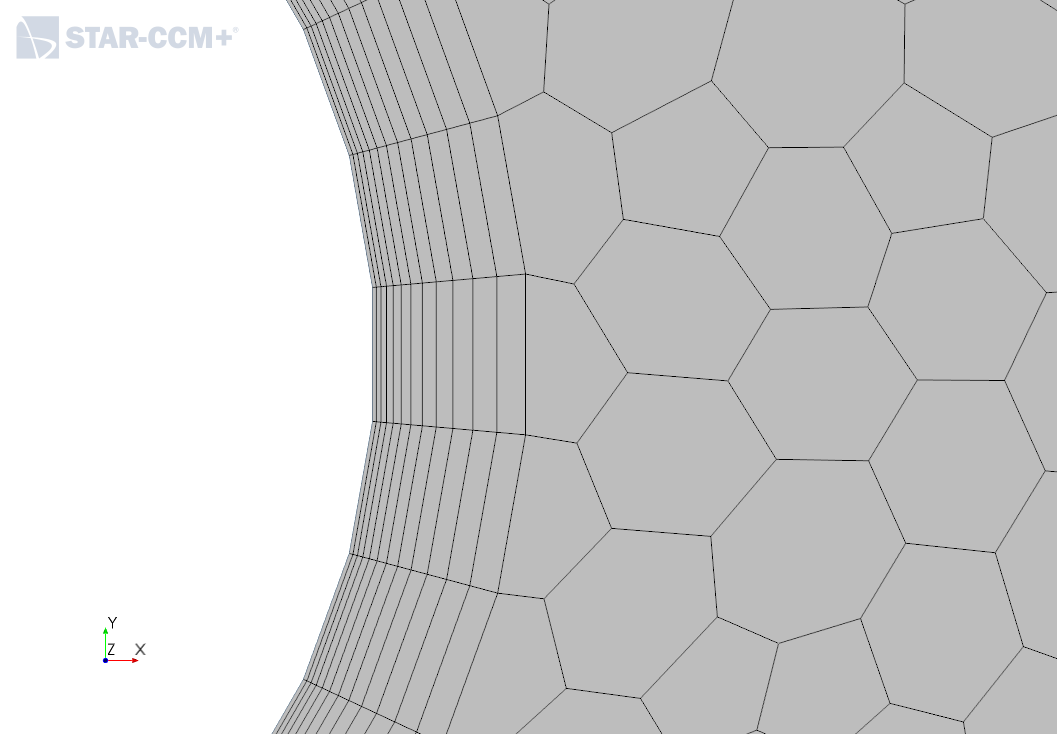
\includegraphics[trim={1.0cm 0cm 1.4cm .5cm},clip,width=0.98\textwidth]{cylinder_2_05_MeshScene2_3.png}
\caption{\vspace{0pt} Cell growth from prism layers to unstructured mesh is course though adequate for the baseline mesh.}
\label{f:mesh05_3}
\end{minipage}
\end{figure}
 
 Because I had the luxury of using a 32 core workstation, I was able to tune the temporal parameters on the fly.  I found that the steady state solution as shown by both the force time history as well as the average vorticity in the domain occurred in 5 seconds for Re 150 and 15 seconds for Re 20.  These model times correspond to allowing a particle in the wake traverse the entire domain 2.5x for Re 150 and 1.1x for Re 20.  Plots of these time histories can be seen in \crefrange{f:Ave_150}{f:CD_time_20} in Appendix A.  I changed the inner iterations parameter between 2 and 10 iterations and found 6 to be adequate.  I also changed the time step from 0.1 to 0.0005 and found 0.005 to be adequate.  With this simulation, I calculated the drag coefficient for both Reynolds numbers and found the agreement to the experimental data to be excellent as discussed above.  \Cref{f:scalar05_1} shows the velocity response and clearly shows the Von-Karman vortex shedding into the wake. 
 
 \begin{figure}[h]
\centering
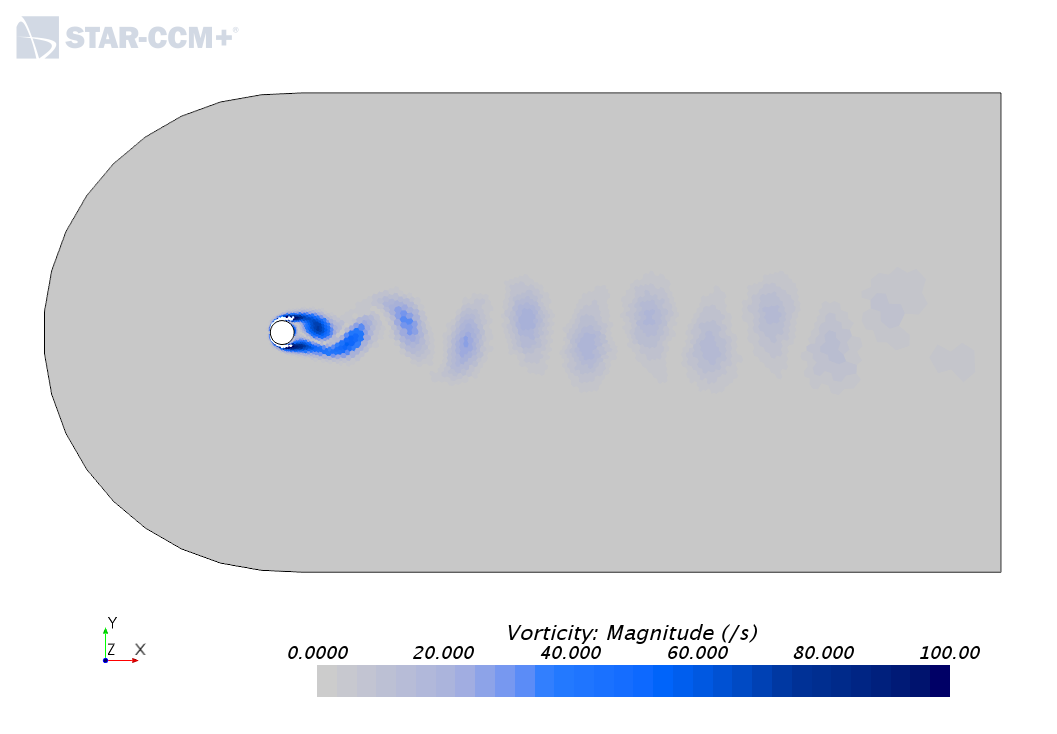
\includegraphics[trim={1.5cm 0cm 1.0cm 3cm},clip,width=0.8\textwidth]{cylinder_2_05_ScalarScene2_Re150.png}
\vspace{-5pt}
\caption{Initial simulation vorticity magnitude shows that a relatively coarse wake mesh is adequate at resolving forces on the cylinder body. }
\label{f:scalar05_1}
\end{figure}

In addition to the drag coefficient validation, I calculated the frequency of shedding and compared it to the analytical solution for the flow Reynolds and Strouhal numbers.  This version of the simulation gives a frequency of 4.08 Hz while the analytical solution gives 3.9 Hz.  With a very good starting point for a simulation that already accurately models the flow, the following grid, boundary, and temporal convergence studies were simple and straightforward.


\section{Grid Independence}

Using the baseline simulation, I changed the grid base size to include a range from 10 diameters down to approximately 0.5 diameters, dividing the base size in half at each step.  \Crefrange{f:grid20}{f:grid150} show the mean drag coefficient with cell number.  The simulations appear to be very close to being grid converged with the finest cell count, however the next to last finest mesh with a base size of 0.0125 m, or approximately 45,400 cells performed nearly as well and has significantly less computational cost.  For the Re 20 simulation, a much coarser discretization was adequate partly due to the symmetric, steady state, and non-transient nature of the simulation, and partially due to the much lower vorticity.  For time considerations in light of the purpose of this study, I chose the next to last discretization as my baseline mesh going forward.  

\begin{figure}[h!]
\centering
\begin{minipage}{.47\textwidth}
  \centering
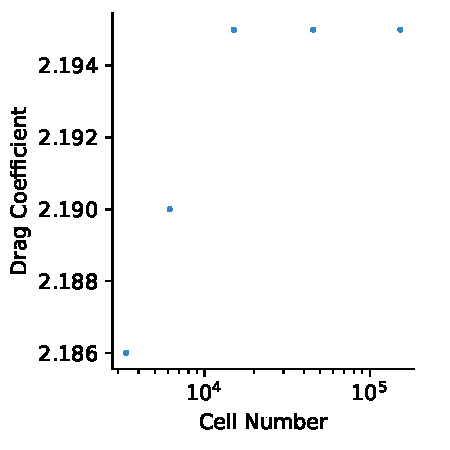
\includegraphics[trim={0.0cm 0cm 0.0cm 0cm},clip,width=0.98\textwidth]{grid20}
\vspace{3pt}
\caption{Re 20 case becomes grid independent with just over 10,000 cells.}
\label{f:grid20}
\end{minipage}%
\hspace{10pt}
\begin{minipage}{.47\textwidth}
  \centering
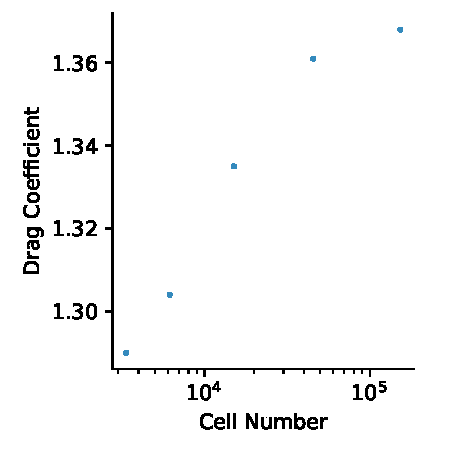
\includegraphics[trim={0.0cm 0cm 0.0cm 0cm},clip,width=0.98\textwidth]{grid150}
\caption{Re 150 case becomes grid independent with slightly more than 300,000 cells}
\label{f:grid150}
\end{minipage}
\end{figure}

\Crefrange{f:cylinder_2_1_MeshScene2}{f:cylinder_2_625_MeshScene2} show the big picture range of mesh discretization from coarsest to finest.  With the discretization I have chosen, the suggested growth rate of 20\% between cells is met, while the wake regions are amply refined.  This enables an efficient distribution of cells in the regions of high vorticity. 

\begin{figure}[h]
\centering
\begin{minipage}{.49\textwidth}
  \centering
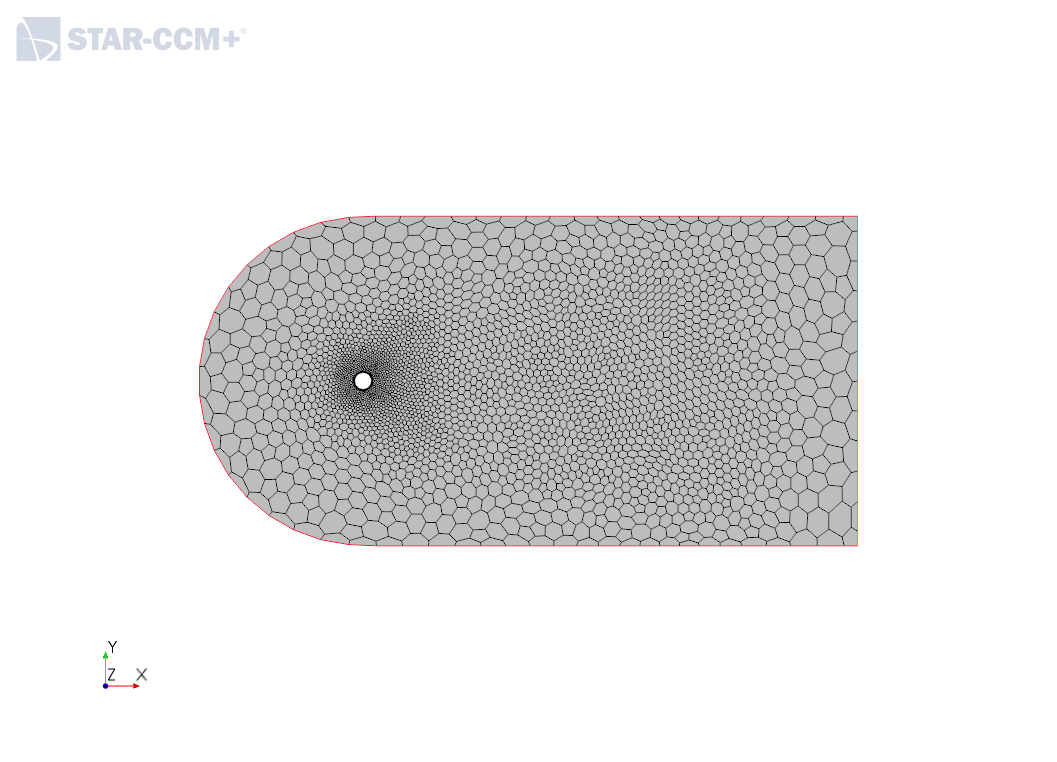
\includegraphics[trim={7.0cm 7.5cm 7.5cm 6.5cm},clip,width=0.98\textwidth]{cylinder_2_1_MeshScene2.png}
%\vspace{-3pt}
\caption{Coarsest mesh consisting of 3,366 cells.}
\label{f:cylinder_2_1_MeshScene2}
\end{minipage}%
\hspace{5pt}
\begin{minipage}{.49\textwidth}
  \centering
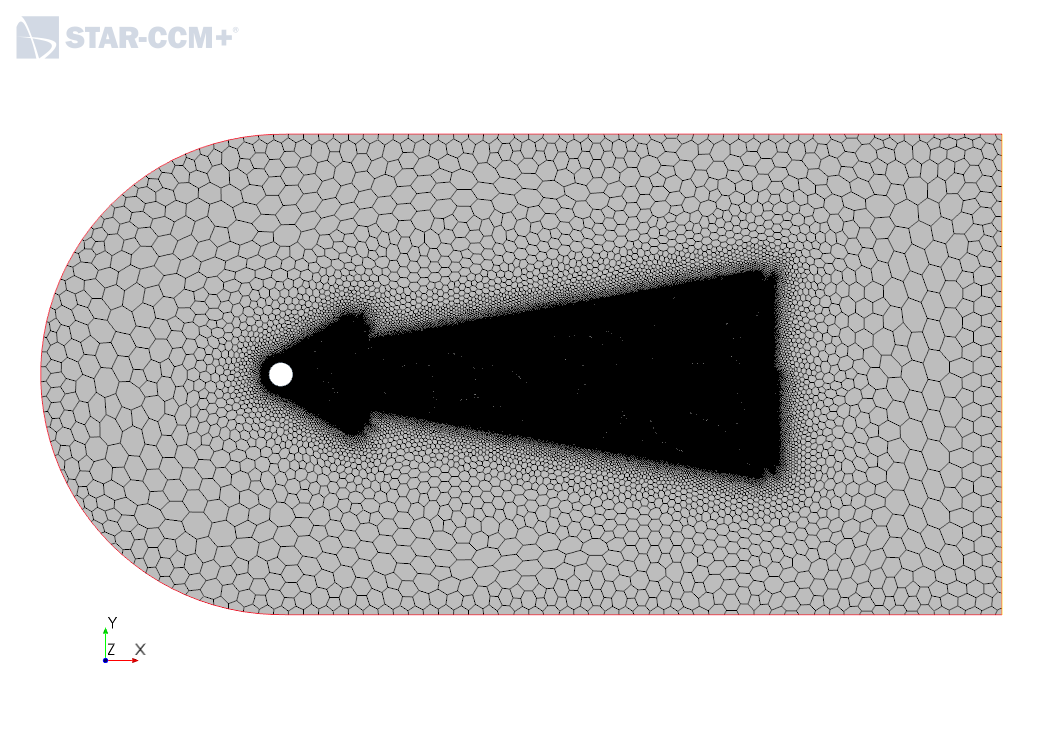
\includegraphics[trim={1.5cm 3.9cm 2.5cm 2.7cm},clip,width=0.98\textwidth]{cylinder_2_625_MeshScene2.png}
\caption{\vspace{0pt}Finest mesh consisting of 153,000 cells.}
\label{f:cylinder_2_625_MeshScene2}
\end{minipage}
\end{figure}

\newpage
\Crefrange{f:cylinder_2_1_MeshScene2_2}{f:cylinder_2_625_MeshScene3} give a closer look at the regions around the cylinder and also in the boundary layer mesh for the coarsest and finest meshes.  Note the fine lateral discretization in \cref{f:cylinder_2_625_MeshScene3} which enabled me to get away with not completely including the full boundary layer thickness in the prism layer mesh for the Re 150 case.  Also shown in \cref{f:cylinder_2_625_MeshScene3}, some slight modifications to the prism layer to unstructured mesh transition would need to be made for a more rigorous study, but for the chosen mesh with a base size of twice the finest mesh, the transition was adequate.  

\begin{figure}[h]
\centering
\begin{minipage}{.49\textwidth}
  \centering
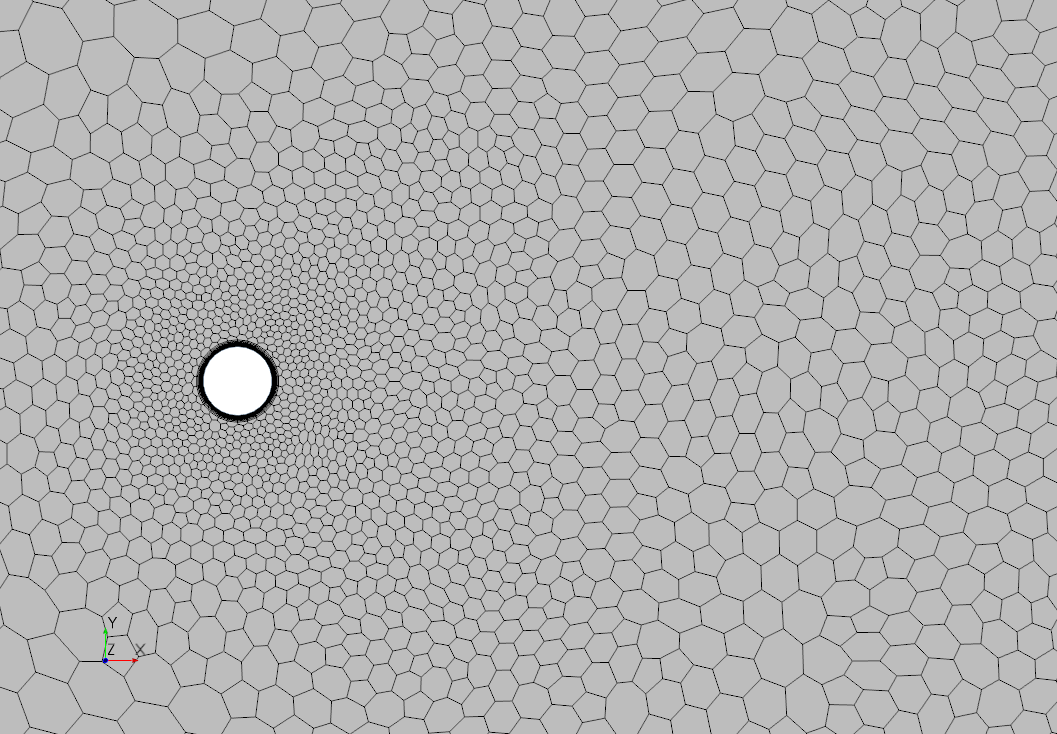
\includegraphics[trim={6.0cm 6cm 13.4cm 6.2cm},clip,width=0.98\textwidth]{cylinder_2_1_MeshScene2_2.png}
%\vspace{-3pt}
\caption{Coarsest mesh includes constant prism layer thickness discretization, but coarse unstructured mesh discretization.}
\label{f:cylinder_2_1_MeshScene2_2}
\end{minipage}%
\hspace{5pt}
\begin{minipage}{.49\textwidth}
  \centering
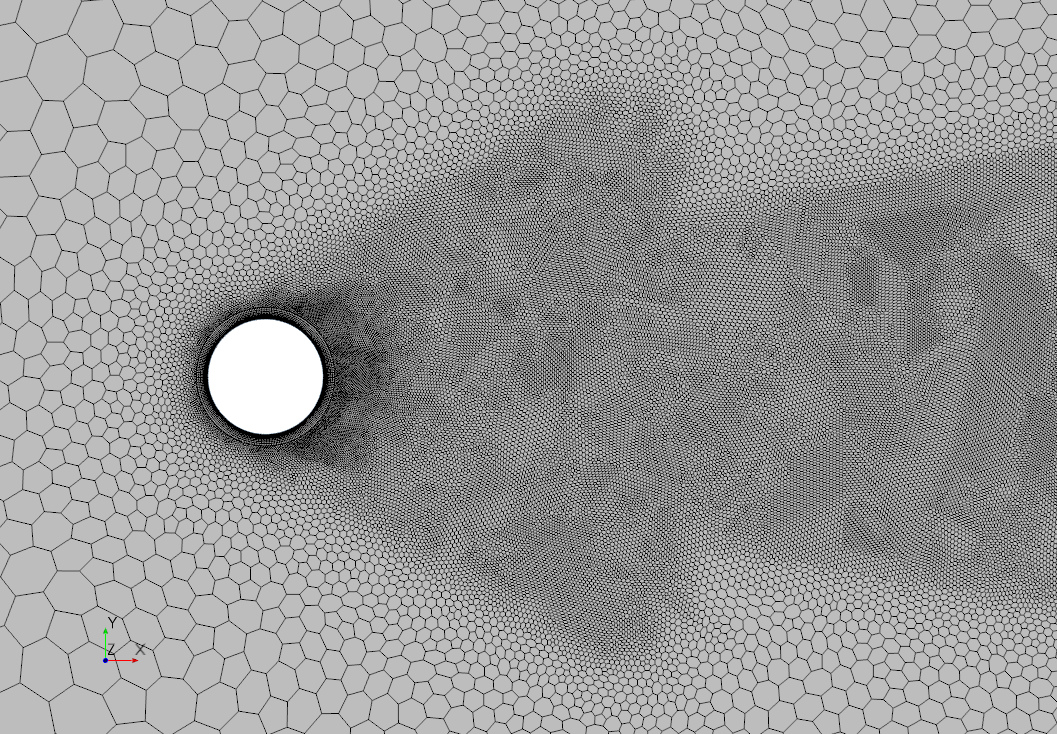
\includegraphics[trim={2.0cm 0cm 2.9cm .5cm},clip,width=0.98\textwidth]{cylinder_2_625_MeshScene2_2.png}
\caption{\vspace{00pt}Finest mesh, note the very fine mesh surrounding the cylinder.}
\label{f:cylinder_2_625_MeshScene2_2}
\end{minipage}
\end{figure}

\begin{figure}[h]
\centering
\begin{minipage}{.49\textwidth}
  \centering
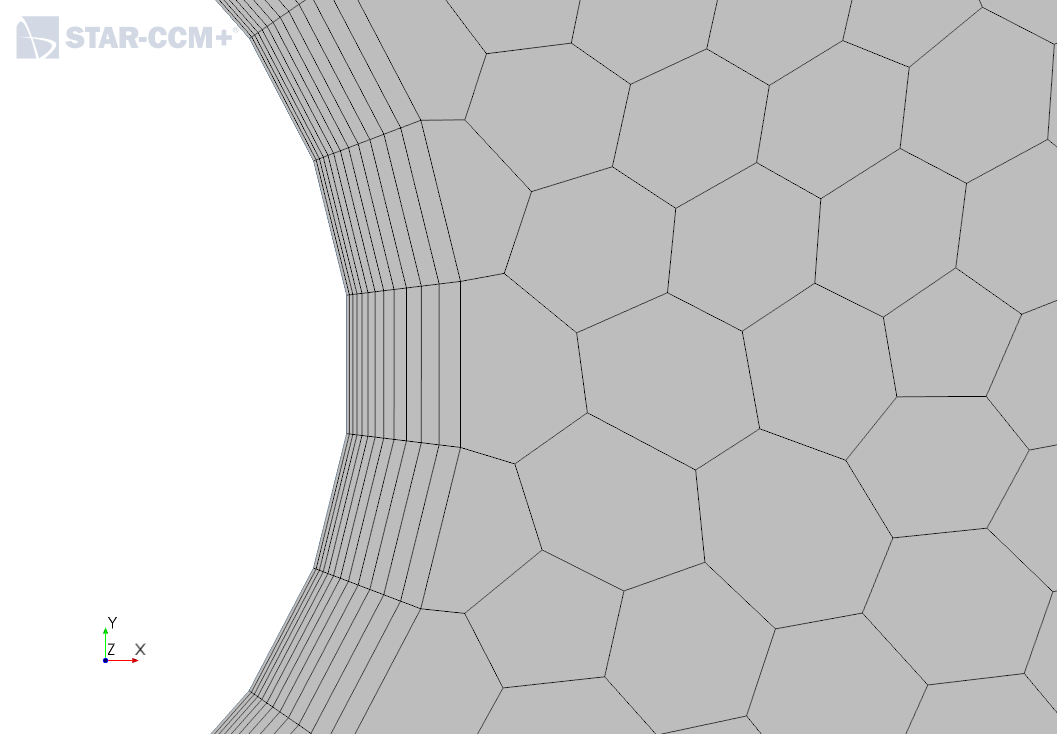
\includegraphics[trim={2.0cm 0cm 2.5cm .5cm},clip,width=0.98\textwidth]{cylinder_2_1_MeshScene3.png}
%\vspace{-3pt}
\caption{Coarsest prism mesh shows poor transition into unstructured mesh.}
\label{f:cylinder_2_1_MeshScene3}
\end{minipage}%
\hspace{5pt}
\begin{minipage}{.49\textwidth}
  \centering
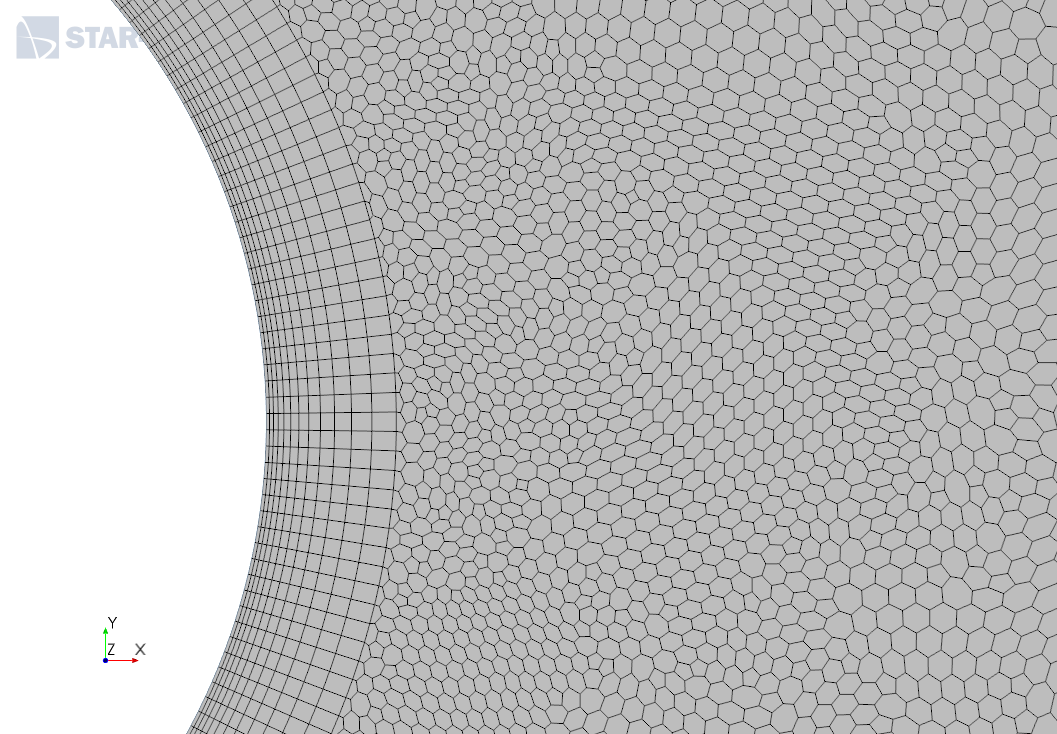
\includegraphics[trim={2.0cm 0cm 2.5cm .5cm},clip,width=0.98\textwidth]{cylinder_2_625_MeshScene3.png}
\caption{\vspace{0pt}Finest prism mesh shows transition into the unstructured mesh to be slightly too fine.}
\label{f:cylinder_2_625_MeshScene3}
\end{minipage}
\end{figure}


\section{Boundary Independence}

While conducting the boundary independence study, it became apparent that my inlet condition of velocity in the x-direction across the entire continuous inlet surface may not have been the best for this study.  With the cylinder splitting the flow in the center of the domain, it is likely that a pressure boundary condition on the upper and lower surfaces would have allowed the slight y-direction flow and would have needed a smaller inlet radius.  As it is, a very large inlet radius was required with my chosen boundary condition to become boundary independent.  After testing up to a radius of 18 diameters, I estimated that a radius of 22 diameters would be necessary, but due to time constraints on the study I chose a radius of 16 diameters.  (See \crefrange{f:boundary20}{f:boundary150}.)  I found this boundary distance to be adequate for force calculations.  A to-scale image of the chosen domain of 16 diameters inlet radius is found in \cref{f:domain}.

\begin{figure}[h!]
\centering
\begin{minipage}{.47\textwidth}
  \centering
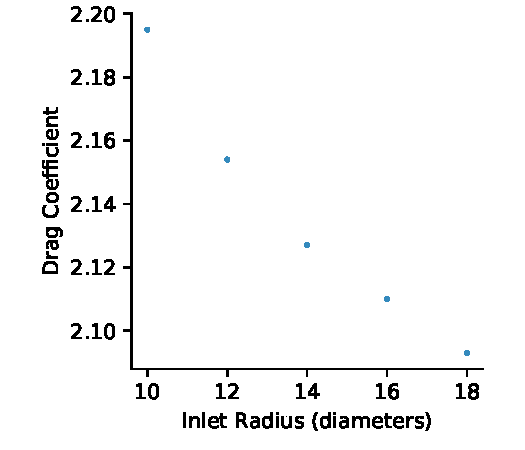
\includegraphics[trim={0.0cm 0cm 0.0cm 0cm},clip,width=0.98\textwidth]{boundary20}
\vspace{3pt}
\caption{Re 20 case becomes boundary independent with a inlet radius of just over 20 diameters.}
\label{f:boundary20}
\end{minipage}%
\hspace{10pt}
\begin{minipage}{.47\textwidth}
  \centering
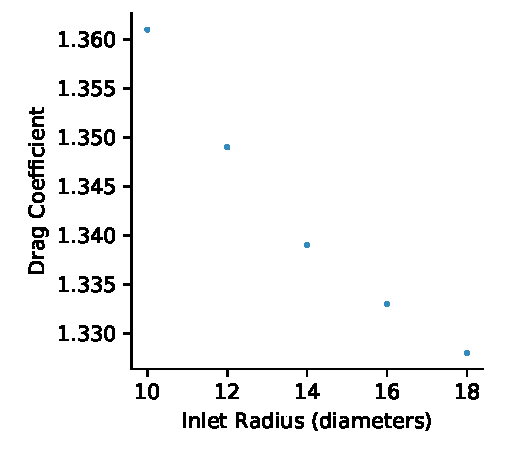
\includegraphics[trim={0.0cm 0cm 0.0cm 0cm},clip,width=0.98\textwidth]{boundary150}
\caption{Re 150 case becomes boundary independent with a inlet radius of just over 20 diameters.}
\label{f:boundary150}
\end{minipage}
\end{figure}



\section{Temporal/Solver Independence}

With the mesh and boundary studies finished and a reasonable domain chosen, I more formally revisited the temporal and solver criteria for the Re 150 case.  Again, for the Re 20 case, the solution has no oscillation, is not affected by temporal parameters, and consequently is not included in this section.  My time step up until now was 0.005 seconds, so I doubled it then iteratively halved it until 0.00125 seconds.  The second order temporal time solver is being used for these simulations.  As shown in \cref{f:timestep150}, a timestep of 0.0025 seconds became temporally independent.  On a side note, if I increased the time step above 0.01, I began to see significant numerical damping which removed the vortex shedding altogether.  

\Cref{f:II150} shows the results of the final condition I changed in this study, the inner iterations.  The number of inner iterations is the number of time-frozen steps the solver takes to converge between time steps.  I found that 6 was adequate and was unchanged from my original simulation.  

\begin{figure}[h!]
\centering
\begin{minipage}{.47\textwidth}
  \centering
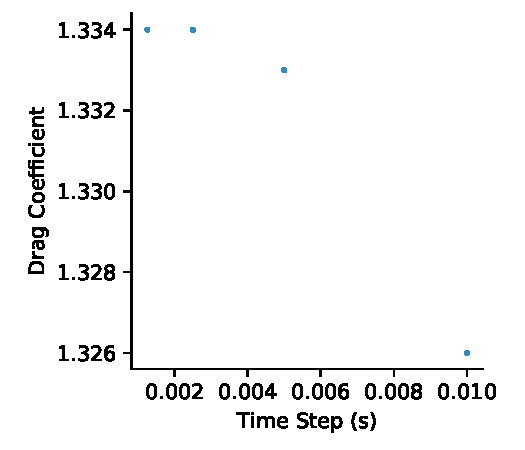
\includegraphics[trim={0.0cm 0cm 0.0cm 0cm},clip,width=0.98\textwidth]{timestep150}
\vspace{3pt}
\caption{Timestep of 0.0025 was adequate for temporal convergence (Re 150 case).}
\label{f:timestep150}
\end{minipage}%
\hspace{10pt}
\begin{minipage}{.47\textwidth}
  \centering
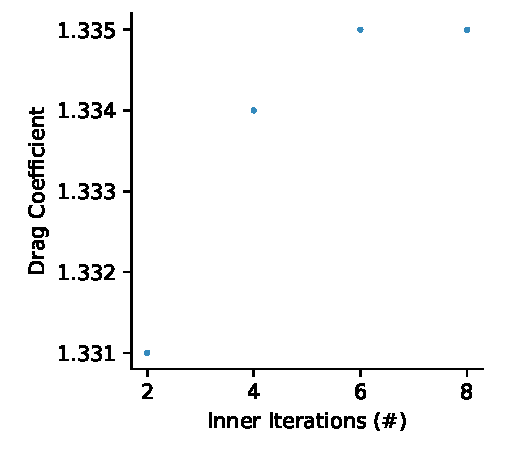
\includegraphics[trim={0.0cm 0cm 0.0cm 0cm},clip,width=0.98\textwidth]{II150}
\caption{Six inner iterations were adequate for solver convergence (Re 150 case).}
\label{f:II150}
\end{minipage}
\end{figure}

\newpage
\section{Conclusions}

I was pleased with the outcomes of the study in that: First the results were quite close to real data.  Second, the convergence and independency studies followed normal asymptotical trends.  Third, the final solution simulation which was deemed adequate by the studies was still simple enough to run in a reasonable amount of time.  \Cref{tab:chosen_sim} gives a brief summary of the main parameters used for the final simulation. A skeleton Star-CCM+ .sim and also an html file containing all of the simulation settings can be found at: \href{https://github.com/moore54/ME541.git}{https://github.com/moore54/ME541.git}.

\begin{table*}[h]
\vspace{20pt}
\centering
  \begin{tabular}{lll}
    \textbf{Name} & \textbf{Value} & \textbf{Description}  \\
    Base Size & 0.0125 m & Mesh base size for which scaling is based upon  \\
    Li & 16 D & Inlet Radius\\
    Ts & 0.0025 s & Temporal discretization\\
    Inner Iterations & 5 & Number of iterations at each time step\\
    Prism Layers & 12 & Number of boundary cells designed to resolve boundary layers\\
    Prism Layer Thickness & 0.001 m & Total thickness of prism layer cells\\
    Prism Layer Minimum Thickness & 2.5E-4 m & Minimum prism cell thickness\\ 
    Temporal Solver Scheme & Second Order & Method for which temporal discretization is solved\\
    Fluid Type & Constant Density & Solver fluid assumptions\\
    Fluid Flow & Laminar & Solver fluid assumptions\\
    Lw & 30 D & Outlet Distance\\
    Lrw & 20 D & Resolved Wake Distance\\
    Re & 20, 150 & Reynolds Number (cylinder diameter)\\
    $\rho$  & 1.225 m/kg & Fluid Density\\
    $\mu$  & 1.855 E-5 Pa-s & Fluid Viscosity\\ 
  \end{tabular}
  \caption{Summary of simulation parameters chosen as an adequate case for the given objective. A skeleton Star-CCM+ .sim file for my final simulation and an html file containing all of the simulation settings can be found at: \href{https://github.com/moore54/ME541.git}{https://github.com/moore54/ME541.git}}
  \label{tab:chosen_sim}
\end{table*}

The ending Von Karman frequency turned out to be 4.18 Hz, slightly larger than the original simulation's 4.08 Hz, and somewhat larger than the analytical 3.9 Hz.  I did find though that by decreasing the time step and increasing the number of inner iterations, the frequency was lowered slightly.  If my objective in this study was to accurately resolve the wake frequency characteristics as opposed to just the wake structure and resulting forces, a much more rigorous study would need to be made with experimental Von Karman wake data.

\section{Star-CCM+ Tutorials}

   While I did not complete any tutorials for this assignment, I have had previous experience with Star-CCM+ and 2D incompressible flows.  The tutorials on moving reference frame and transient fan simulations would be of interest for single propeller validation studies with wake profiles in mind.  Also, the tutorials on sound modeling could also be useful if I decide to do CFD while creating a sound model for propeller design optimization.  

\section{Appendix A: Final Simulation Overview}

The following figures show the mesh, velocity and vorticity solutions, and time histories for both the Re 20 and Re 150 cases for the chosen simulation parameters.

 \begin{figure}[h]
\centering
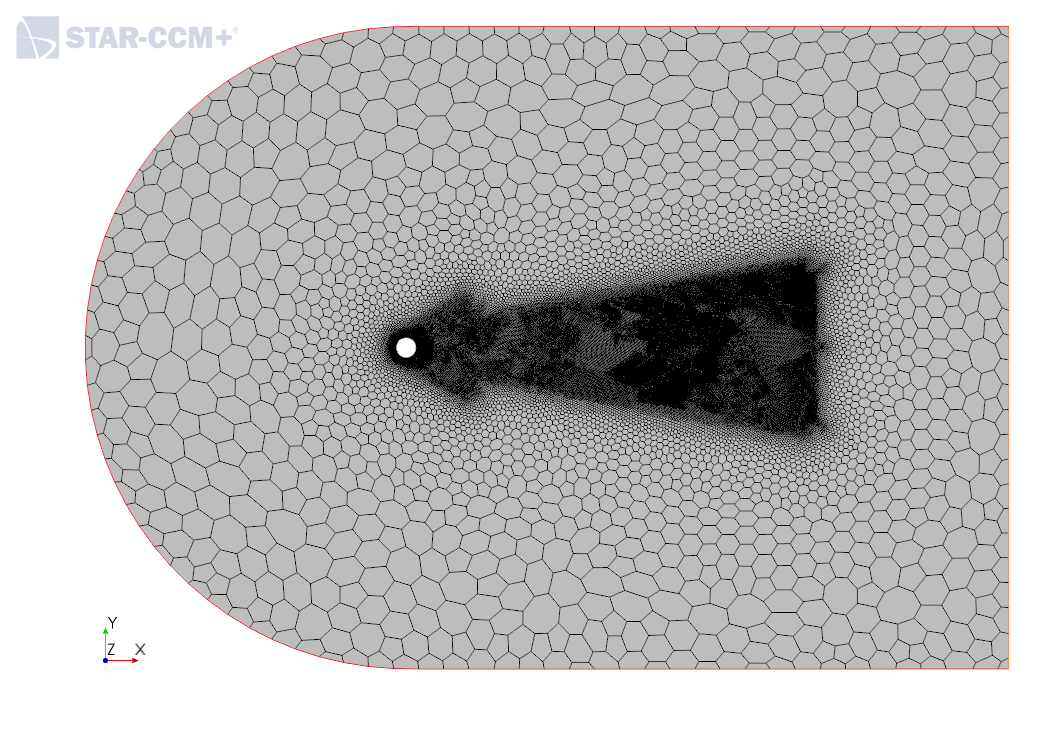
\includegraphics[trim={0.0cm 0cm 0.0cm 0cm},clip,width=0.8\textwidth]{cylinder_2_016_MeshScene2.png}
\vspace{-5pt}
\caption{Final simulation full domain mesh. }
\label{f:cylinder_2_016_MeshScene2}
\end{figure}


\begin{figure}[h]
\centering
\begin{minipage}{.49\textwidth}
  \centering
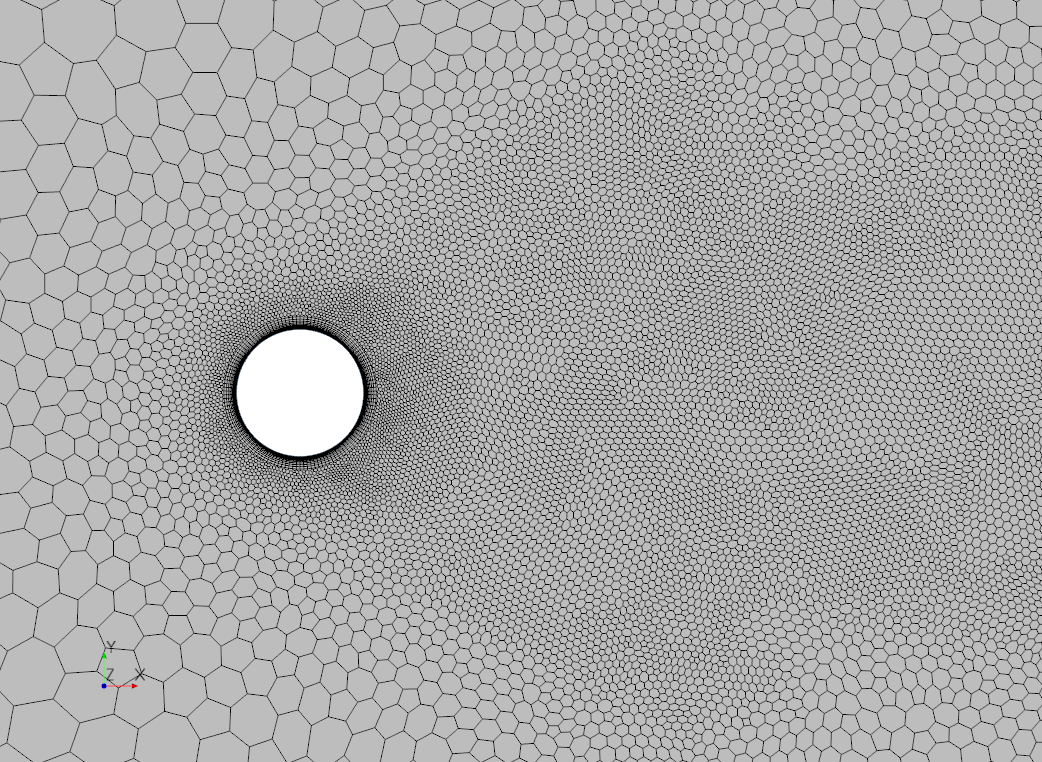
\includegraphics[trim={2.0cm 0cm 2.5cm .5cm},clip,width=0.98\textwidth]{cylinder_2_016_MeshScene2_2.png}
%\vspace{-3pt}
\caption{Final simulation near field mesh.}
\label{f:cylinder_2_016_MeshScene2_2}
\end{minipage}%
\hspace{5pt}
\begin{minipage}{.49\textwidth}
  \centering
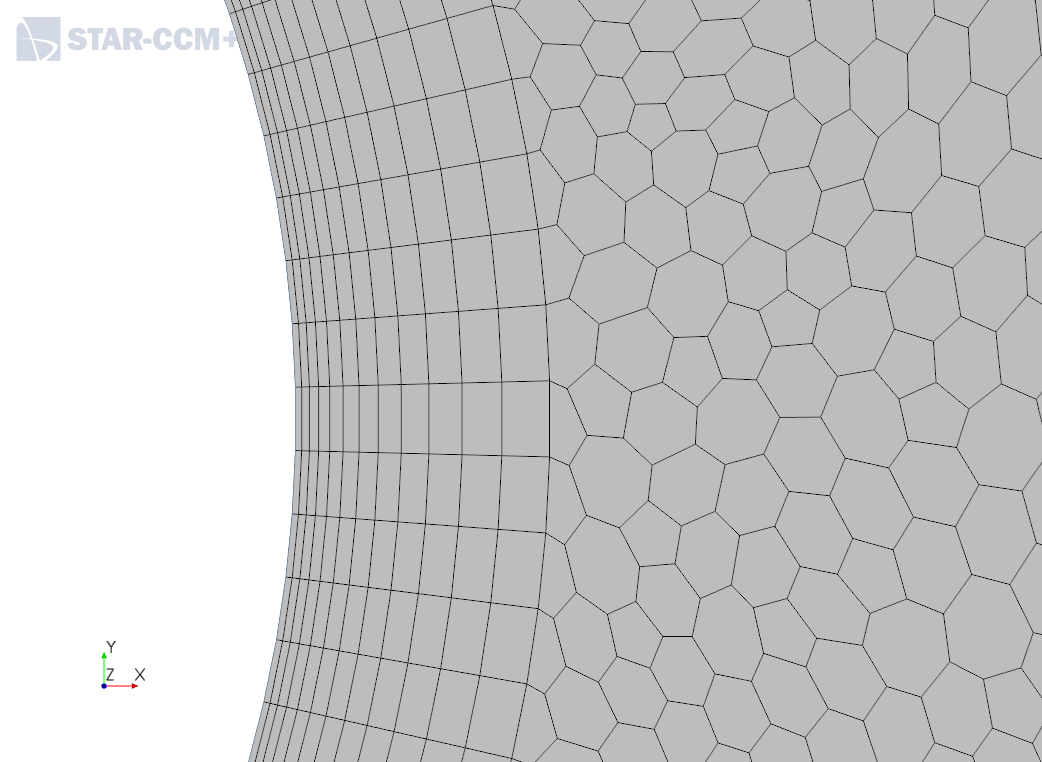
\includegraphics[trim={2.0cm 0cm 2.5cm .5cm},clip,width=0.98\textwidth]{cylinder_2_016_MeshScene2_3.png}
\caption{\vspace{0pt}Final simulation boundary layer mesh.}
\label{f:cylinder_2_016_MeshScene2_3}
\end{minipage}
\end{figure}

 \begin{figure}[h]
\centering
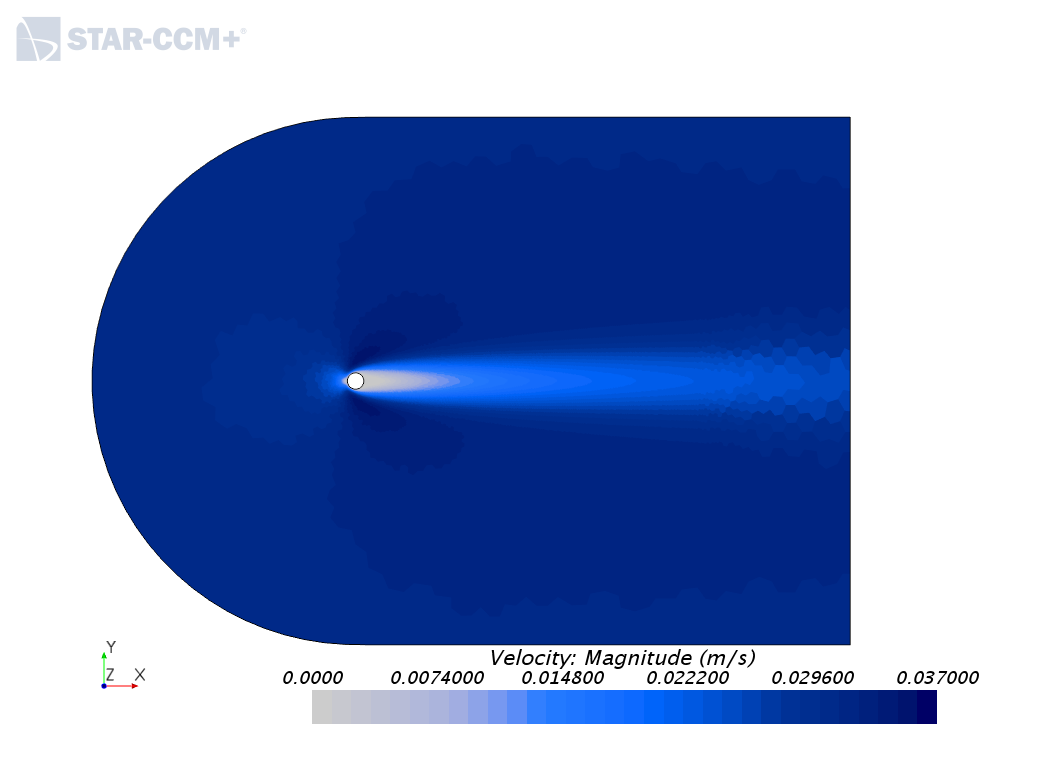
\includegraphics[trim={0.0cm 0cm 0.0cm 0cm},clip,width=0.9\textwidth]{cylinder_2_016_ScalarScene1_re20.png}
\vspace{-5pt}
\caption{Final simulation velocity field Re 20.}
\label{f:cylinder_2_016_ScalarScene1_re20}
\end{figure}

 \begin{figure}[h]
\centering
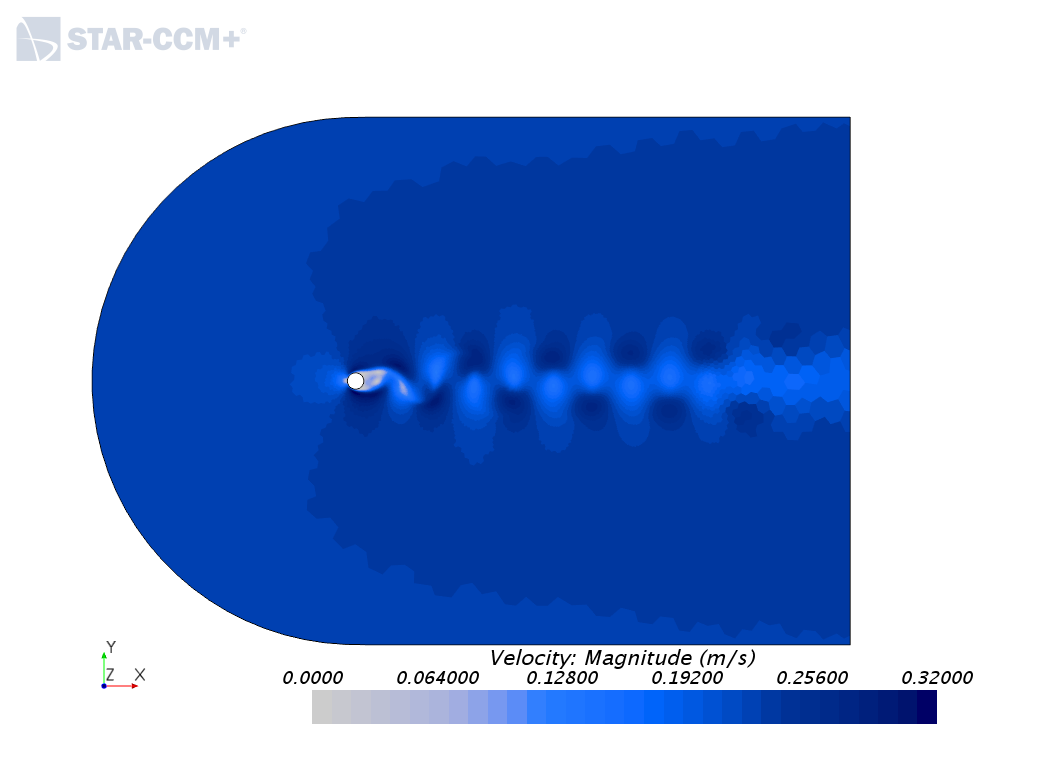
\includegraphics[trim={0.0cm 0cm 0.0cm 0cm},clip,width=0.9\textwidth]{cylinder_2_016_ScalarScene1.png}
\vspace{-5pt}
\caption{Final simulation velocity field Re 150. }
\label{f:cylinder_2_016_ScalarScene1}
\end{figure}

 \begin{figure}[h]
\centering
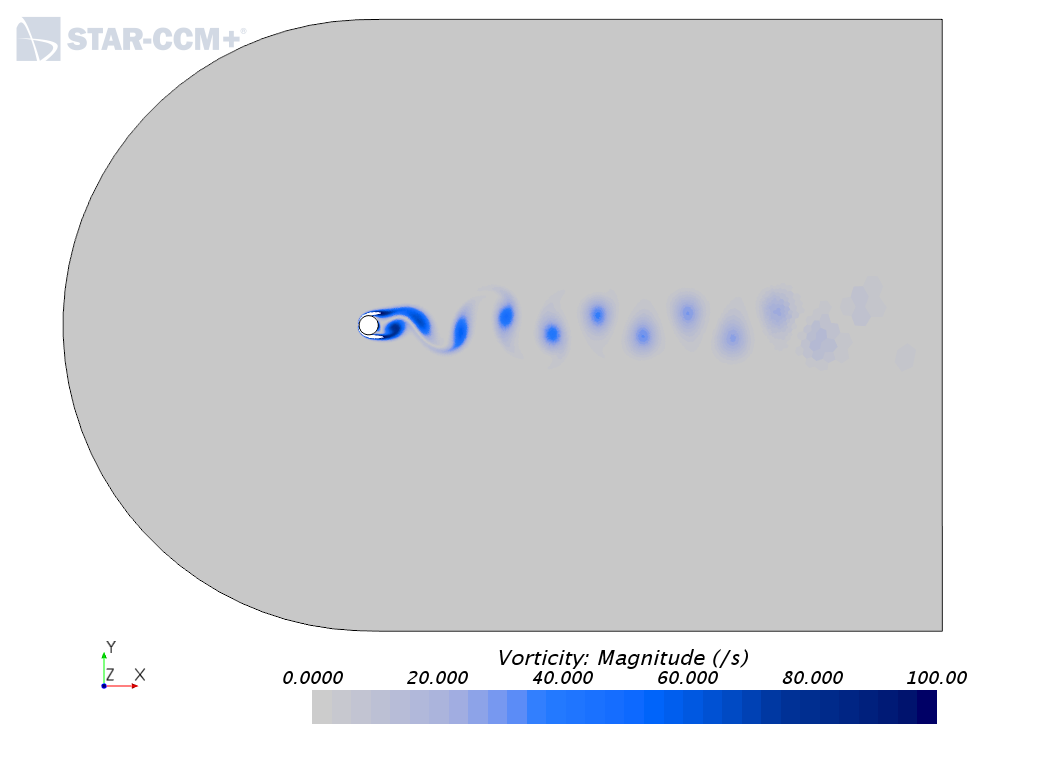
\includegraphics[trim={0.0cm 0cm 0.0cm 0cm},clip,width=0.9\textwidth]{cylinder_2_016_ScalarScene2.png}
\vspace{-5pt}
\caption{Final simulation vorticity field Re 150.}
\label{f:cylinder_2_016_ScalarScene2}
\end{figure}

\begin{figure}[h]
\centering
\begin{minipage}{.49\textwidth}
  \centering
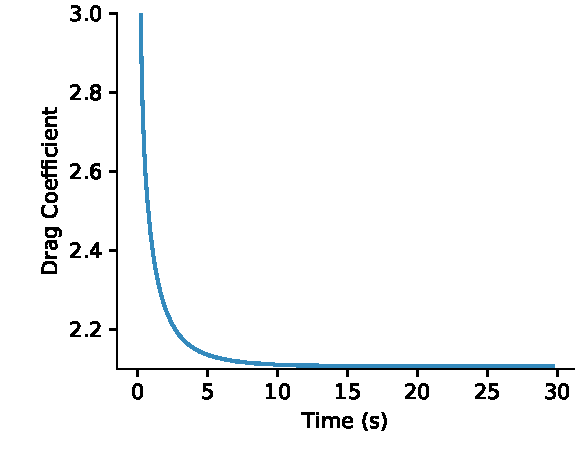
\includegraphics[trim={0.0cm 0cm 0.0cm 0cm},clip,width=0.98\textwidth]{CD_time_20}
%\vspace{-3pt}
\caption{Final simulation drag coefficient as a function of time Re 20.}
\label{f:CD_time_20}
\end{minipage}%
\hspace{5pt}
\begin{minipage}{.49\textwidth}
  \centering
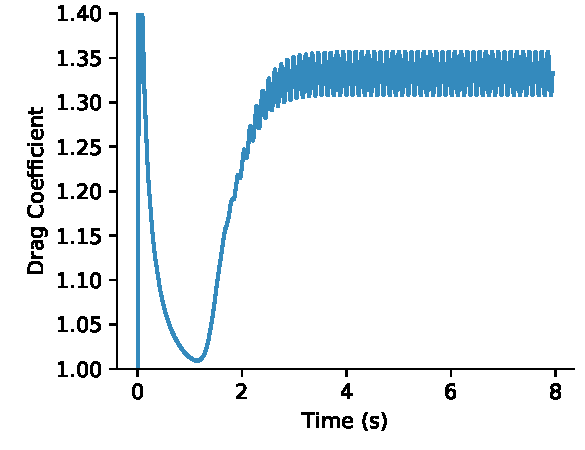
\includegraphics[trim={0.0cm 0cm 0.0cm 0cm},clip,width=0.98\textwidth]{CD_time_150}
\caption{\vspace{0pt}Final simulation drag coefficient as a function of time Re 150.}
\label{f:CD_time_150}
\end{minipage}
\end{figure}

\begin{figure}[h]
\centering
\begin{minipage}{.49\textwidth}
  \centering
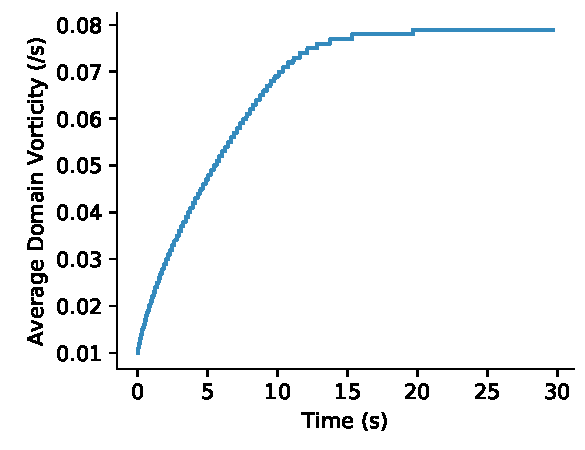
\includegraphics[trim={0.0cm 0cm 0.0cm 0cm},clip,width=0.98\textwidth]{Ave_20}
%\vspace{-3pt}
\caption{Final simulation average fluid domain vorticity as a function of time Re 20.}
\label{f:Ave_20}
\end{minipage}%
\hspace{5pt}
\begin{minipage}{.49\textwidth}
  \centering
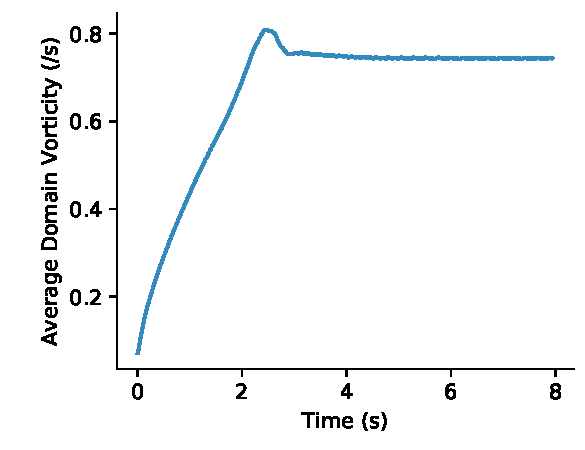
\includegraphics[trim={0.0cm 0cm 0.0cm 0cm},clip,width=0.98\textwidth]{Ave_150}
\caption{\vspace{0pt}Final simulation average fluid domain vorticity as a function of time Re 150.}
\label{f:Ave_150}
\end{minipage}
\end{figure}

\FloatBarrier
\subsection{Wake Development}

\vspace{-5pt}

 \begin{figure}[h]
\centering
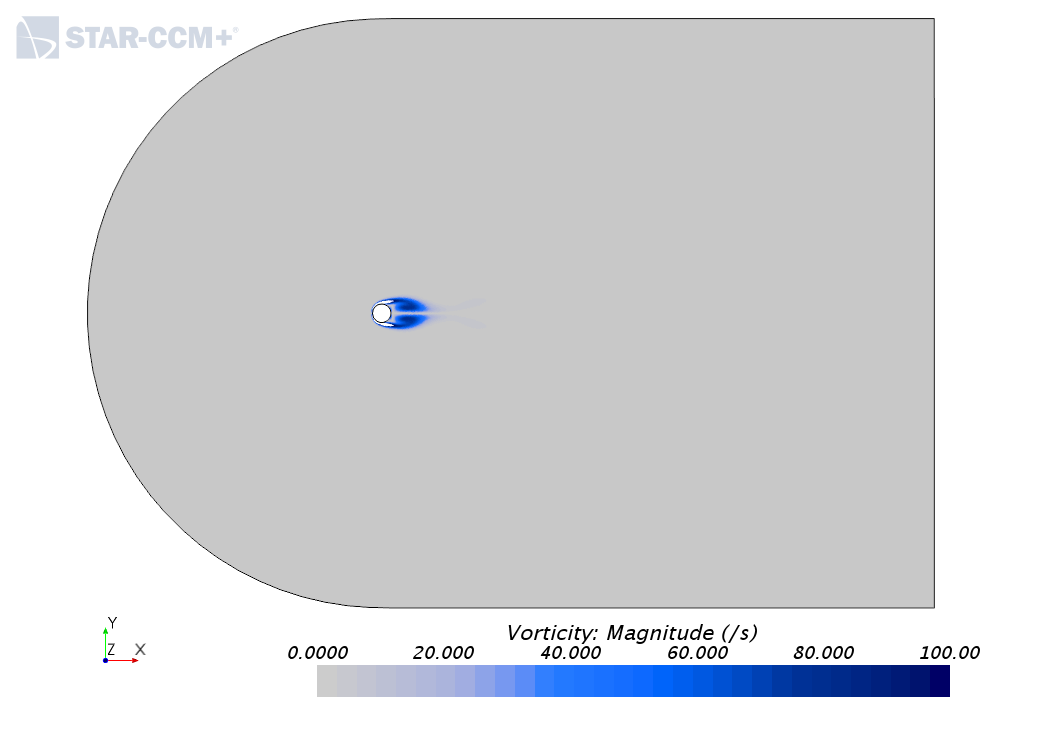
\includegraphics[trim={0.5cm 1.5cm 0.5cm .6cm},clip,width=0.8\textwidth]{start}
\vspace{-5pt}
\caption{Re 150 beginning wake.}
\label{f:start}
\end{figure}

\vspace{-5pt}

 \begin{figure}[h]
\centering
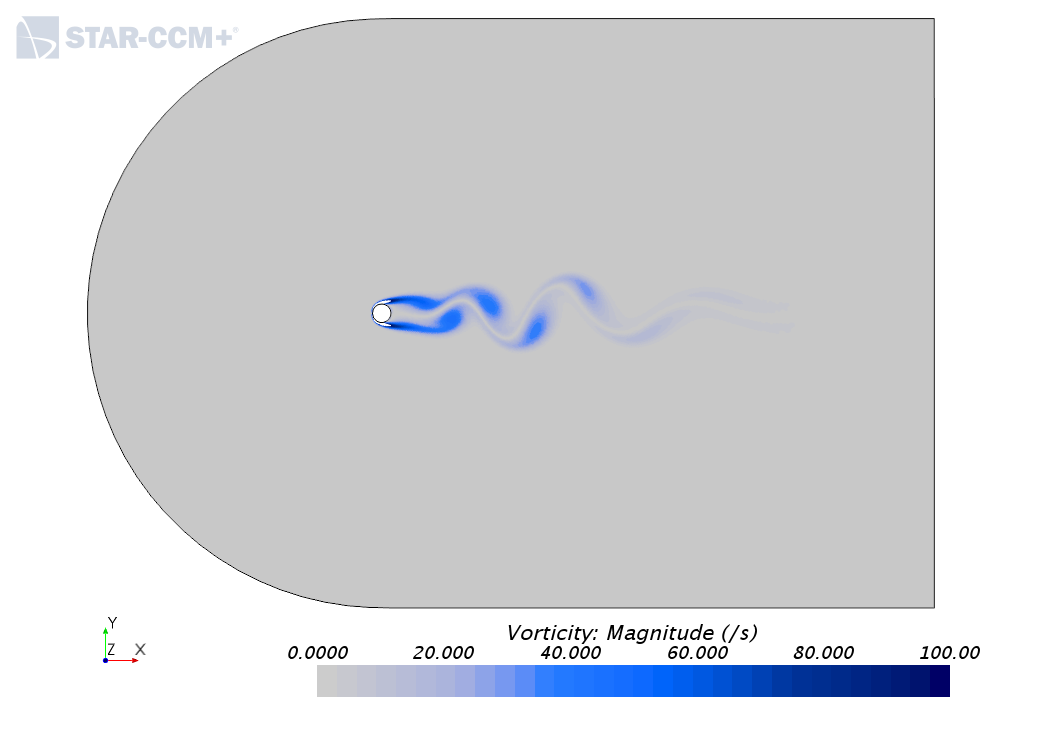
\includegraphics[trim={0.5cm 1.5cm 0.5cm .6cm},clip,width=0.8\textwidth]{mid}
\vspace{-5pt}
\caption{Re 150 mid development wake}
\label{f:mid}
\end{figure}

\vspace{-5pt}

 \begin{figure}[h]
\centering
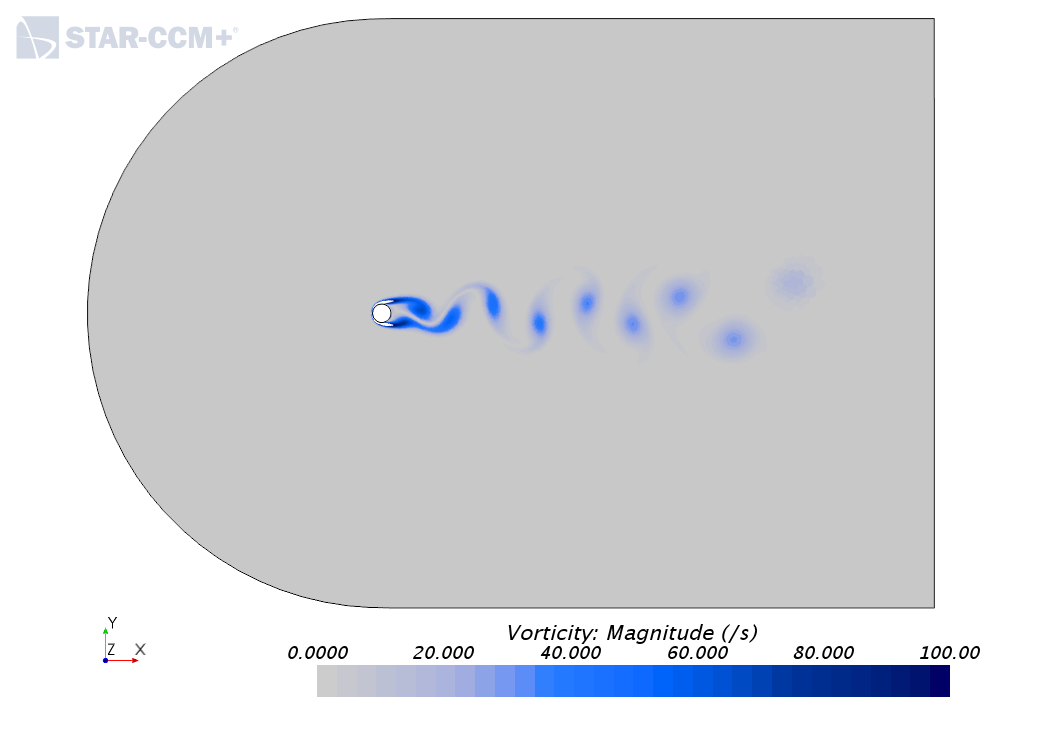
\includegraphics[trim={0.5cm 1.5cm 0.5cm .6cm},clip,width=0.8\textwidth]{nearfull}
\vspace{-5pt}
\caption{Re 150 near full developed wake.}
\label{f:nearfull}
\end{figure}

\vspace{-5pt}

 \begin{figure}[h]
\centering
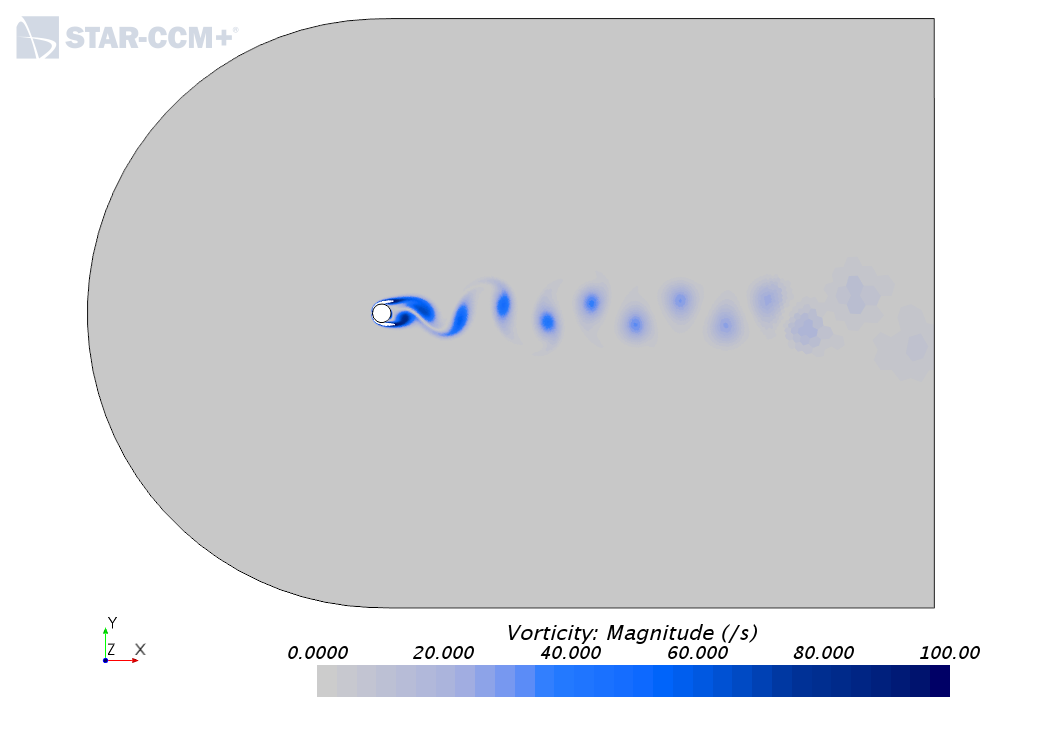
\includegraphics[trim={0.5cm 1.5cm 0.5cm .6cm},clip,width=0.8\textwidth]{full}
\vspace{-5pt}
\caption{Re 150 fully developed wake.}
\label{f:full}
\end{figure}

\vspace{-5pt}

 \begin{figure}[t!]
\centering
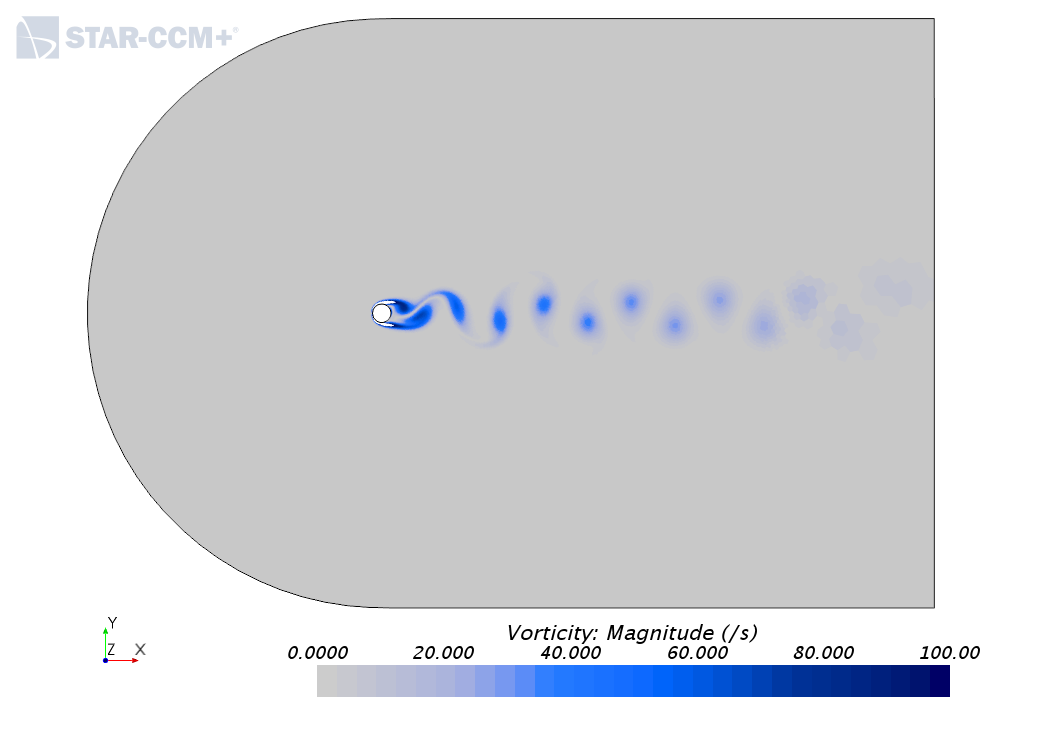
\includegraphics[trim={0.5cm 1.5cm 0.5cm .6cm},clip,width=0.8\textwidth]{after}
\vspace{-5pt}
\caption{Re 150 opposite vortex being shed.}
\label{f:after}
\end{figure}

\end{document}
